% ==========================================
% BAB I PENDAHULUAN
% ==========================================
\chapter{PENDAHULUAN}
\label{chap:pendahuluan}

Bab I adalah pendahuluan yang menceritakan keseluruhan isi dari tugas akhir. Bab ini diawali dengan penjelasan mengenai topik dan latar belakang tugas akhir, dilanjuti dengan rumusan masalah, tujuan tugas akhir, serta batasan masalah yang dibahas di tugas akhir. Selain itu, Bab I akan menjelaskan tentang pendekatan dan metode yang digunakan di metodologi.

% --- Latar Belakang ---
\section{Latar Belakang}
Revolusi digital telah memicu ledakan produksi data; volume data global diproyeksikan akan mencapai 181 zettabyte pada tahun 2025, meningkat drastis dari hanya 2 zettabyte pada tahun 2010 \autocite{idc2025}. Pertumbuhan ini melahirkan tantangan \textit{information overload}, di mana volume informasi melampaui kapasitas kognitif individu untuk memprosesnya \autocite{eppler2004}. Menurut \textit{Cognitive Load Theory}, kapasitas memori kerja manusia yang terbatas membuat kualitas pengambilan keputusan dapat menurun hingga 50\% saat dihadapkan pada beban informasi berlebih \autocite{sweller1988,arnold2023}.

Masalah ini menjadi akut dalam komunitas online di media sosial, di mana laju pesan yang tinggi dapat menenggelamkan informasi krusial \autocite{nematzadeh2019}. Konsekuensinya adalah atensi selektif hingga kelumpuhan dalam pengambilan keputusan \autocite{edmunds2000}. Fenomena ini relevan di Indonesia, di mana platform seperti Telegram telah menjadi ekosistem dominan untuk komunitas finansial berskala besar. Didukung oleh fitur seperti kapasitas grup hingga 200.000 anggota, Telegram menjadi medium pilihan dengan lebih dari 27 juta pengguna di Indonesia untuk diskusi investasi \textit{real-time} \autocite{statista2024,perlo2025}.

Dominasi Telegram ini berjalan paralel dengan lonjakan jumlah investor ritel di Indonesia, yang mencapai lebih dari 6 juta investor pada September 2024, dengan pertumbuhan 744.000 investor baru di tahun tersebut \autocite{bei2024}. Mayoritas investor baru ini adalah generasi muda yang sangat bergantung pada komunitas media sosial untuk pengambilan keputusan investasi \autocite{ojk2022,jema2023}. Ketergantungan ini menciptakan masalah dimana akses informasi justru berujung pada \textit{information overload} yang parah, sehingga investor kesulitan memilah sinyal berkualitas dari kebisingan informasi. Tantangan ini terefleksi secara nyata dalam komunitas finansial Michael Yeoh, yang memiliki lebih dari 22.000 anggota dalam struktur hierarkis empat tingkat (MY Cuap Cuap, MY Swing Plan, MY Advanced Group, dan MY PIRANHA). \textit{Information overload} paling akut terjadi di grup PIRANHA yang terdiri dari 2.000 investor ultra-premium dengan volume diskusi melebihi 200 pesan per jam, di mana fragmentasi informasi antar grup semakin memperburuk masalah.

Penelitian akademis sebelumnya cenderung berfokus pada analisis sentimen dari forum publik seperti X (Twitter) dan Reddit untuk tujuan prediksi pergerakan harga saham (misalnya, \textcite{bollen2011}; \textcite{sianipar2023}; \textcite{liew2021}). Sementara itu, solusi praktis seperti bot Telegram yang ada saat ini bersifat generik, tidak mampu melakukan sintesis lintas-grup, dan tidak dioptimalkan untuk domain finansial Indonesia yang spesifik (misalnya, \textcite{stars2023}; \textcite{panda2023}). Kedua pendekatan tersebut tidak dirancang untuk menyelesaikan masalah operasional internal sebuah komunitas.

Kondisi \textit{information overload} parah dan fragmentasi informasi akibat struktur komunitas berjenjang ini menyoroti permasalahan signifikan yang perlu diteliti. Fenomena ini tidak hanya berisiko mengurangi efektivitas anggota dalam mengambil keputusan investasi, tetapi juga mengikis nilai dari komunitas itu sendiri.

% --- Rumusan Masalah ---
\section{Rumusan Masalah}
Berdasarkan latar belakang yang telah diuraikan pada subbab I.1, rumusan masalah yang akan dibahas pada tugas akhir ini adalah:

\begin{enumerate}
\item Bagaimana merancang dan mengembangkan sistem rangkuman otomatis berbasis \textit{AI} yang dapat mereduksi \textit{information overload} melalui sintesis intelijen lintas-grup dalam komunitas finansial Telegram berjenjang?
\item Bagaimana meningkatkan efektivitas sistem rangkuman otomatis tersebut berdasarkan \textit{feedback} dan evaluasi dari pengguna komunitas?
\end{enumerate}

% --- Tujuan ---
\section{Tujuan}
Berdasarkan latar belakang dan rumusan masalah yang telah dijelaskan, tujuan dari tugas akhir ini adalah:

\begin{enumerate}
\item Merancang, membangun, dan mengevaluasi sistem \textit{prototype} rangkuman otomatis berbasis \textit{AI} yang mampu melakukan sintesis intelijen lintas-grup untuk mereduksi \textit{information overload} dalam komunitas finansial Telegram.
\item Melakukan iterasi perbaikan sistem berdasarkan \textit{feedback} pengguna untuk meningkatkan efektivitas dan \textit{usability} sistem dalam konteks komunitas yang diteliti.
\end{enumerate}

% --- Batasan Masalah ---
\section{Batasan Masalah}
Batasan masalah digunakan untuk menjaga pelebaran dari pokok masalah dan mengarahkan tugas akhir menjadi lebih spesifik. Batasan masalah dari tugas akhir ini adalah:

\begin{enumerate}
\item Konteks penelitian dan implementasi sistem terbatas secara eksklusif pada ekosistem komunitas investasi Michael Yeoh di Telegram, yang terdiri dari empat grup berjenjang: MY Cuap Cuap (~18.000 anggota, \textit{read-only} untuk informasi umum), MY Swing Plan (grup sinyal \textit{trading} dengan format terstruktur), MY Advanced Group (~4.000 anggota premium dengan komunikasi interaktif dua arah), dan MY PIRANHA (~2.000 anggota ultra-premium dengan volume diskusi tertinggi melebihi 200 pesan per jam).

\item Arsitektur sistem menggunakan tumpukan teknologi (\textit{technology stack}) yang telah ditentukan, meliputi model NLP \textit{cahya/bert-base-indonesian-NER} untuk ekstraksi entitas finansial, \textit{indonesian-roberta-base-emotion-classifier} untuk analisis emosi, BERTopic untuk pemodelan topik, serta pemanfaatan Groq API dengan model bahasa Llama 3.1 70B untuk proses generasi rangkuman.

\item Keluaran (\textit{output}) utama dari sistem adalah rangkuman terstruktur yang dihasilkan secara periodik setiap jam (11:00, 12:00, 14:00, 15:00, 16:00) sebagai suplemen rangkuman manual resmi yang ada. Penelitian ini tidak mencakup pengembangan sistem peringatan (\textit{alert}) \textit{real-time} atau fitur percakapan interaktif.

\item Sumber data untuk analisis terbatas pada pesan berbasis teks yang ada di dalam grup-grup Telegram yang ditentukan. Sistem tidak mengintegrasikan sumber data eksternal seperti API harga saham \textit{real-time} atau umpan berita finansial dari portal media.

\item Sistem menerapkan prinsip privasi dengan TIDAK memproses pesan yang telah di-\textit{unsend} oleh pengirim, mengakui bahwa tindakan \textit{unsend} merupakan indikasi eksplisit penarikan kembali informasi dari domain publik komunitas. Implementasi ini memastikan bahwa hanya konten yang secara sadar dipublikasikan secara permanen oleh anggota yang akan dianalisis oleh sistem.
\end{enumerate}

% --- Metodologi Pengerjaan TA ---
\section{Metodologi}
Pengerjaan tugas akhir ini menggunakan dua metodologi, yaitu metodologi untuk penelitian dan metodologi pengembangan.

\subsection{Metodologi Penelitian}
Metodologi penelitian yang digunakan adalah \textit{Design Science Research Methodology} (DSRM). Pendekatan DSRM dipilih karena relevansinya yang tinggi dengan penelitian di bidang sistem informasi yang bertujuan untuk merancang dan mengevaluasi artefak teknologi inovatif guna memecahkan masalah di dunia nyata. Proses DSRM terdiri dari enam tahapan yang akan diikuti dalam penelitian ini:

\begin{enumerate}
\item \textbf{Identifikasi Masalah \& Motivasi}: Tahap ini telah diuraikan dalam latar belakang, di mana masalah spesifik yang diidentifikasi adalah \textit{information overload} dan fragmentasi informasi dalam komunitas finansial Telegram yang besar dan berjenjang. Motivasi utamanya adalah kebutuhan untuk meningkatkan efisiensi akses informasi bagi anggota komunitas.

\item \textbf{Perumusan Tujuan Solusi}: Berdasarkan masalah yang ada, tujuan solusi didefinisikan secara kuantitatif dan kualitatif. Tujuan utamanya adalah menghasilkan sebuah artefak (sistem) yang terbukti mampu mereduksi beban informasi, yang akan diukur melalui akurasi identifikasi topik dan efisiensi akses informasi yang dirasakan pengguna.

\item \textbf{Desain \& Pengembangan}: Tahap ini merupakan aktivitas inti dalam menciptakan artefak penelitian. Pada tugas akhir ini, artefak yang dirancang dan dikembangkan adalah sebuah sistem purwarupa untuk rangkuman otomatis. Proses ini mencakup perancangan arsitektur, implementasi \textit{pipeline} pemrosesan data, dan integrasi model \textit{NLP}.

\item \textbf{Demonstrasi}: Pada tahap ini, artefak yang telah dibangun akan didemonstrasikan untuk menyelesaikan masalah yang telah diidentifikasi. Sistem purwarupa akan dioperasikan menggunakan data percakapan nyata dari komunitas Michael Yeoh untuk menunjukkan kemampuannya dalam mengubah data mentah menjadi rangkuman yang terstruktur.

\item \textbf{Evaluasi}: Artefak akan dievaluasi secara sistematis untuk mengukur sejauh mana tujuan solusi tercapai. Evaluasi akan membandingkan kondisi sebelum dan sesudah penggunaan sistem, menggunakan metrik yang telah ditetapkan seperti akurasi, tingkat kompresi pesan, dan umpan balik kualitatif dari pengguna melalui survei.

\item \textbf{Komunikasi}: Tahap terakhir adalah mengkomunikasikan masalah, artefak yang dibangun, serta hasil evaluasinya kepada audiens akademis. Komunikasi ini diwujudkan melalui penulisan laporan tugas akhir ini serta presentasi dalam forum seminar dan sidang.
\end{enumerate}

\subsection{Metodologi Pengembangan}
Metodologi pengembangan yang digunakan dalam penelitian ini adalah \textit{Cross Industry Standard Process for Data Mining} (CRISP-DM). Metodologi CRISP-DM dipilih karena relevansinya yang tinggi untuk proyek berbasis \textit{machine learning} dan \textit{natural language processing}, serta kemampuannya dalam memberikan kerangka kerja terstruktur untuk proyek \textit{data mining} di berbagai industri \autocite{chapman2000}. CRISP-DM terdiri dari enam fase utama yang bersifat iteratif dan siklik, memungkinkan pengulangan dan penyempurnaan di setiap tahap pengembangan. Metodologi CRISP-DM dapat dilihat pada Gambar \ref{fig:crisp-dm}.

\begin{figure}[H]
  \centering
  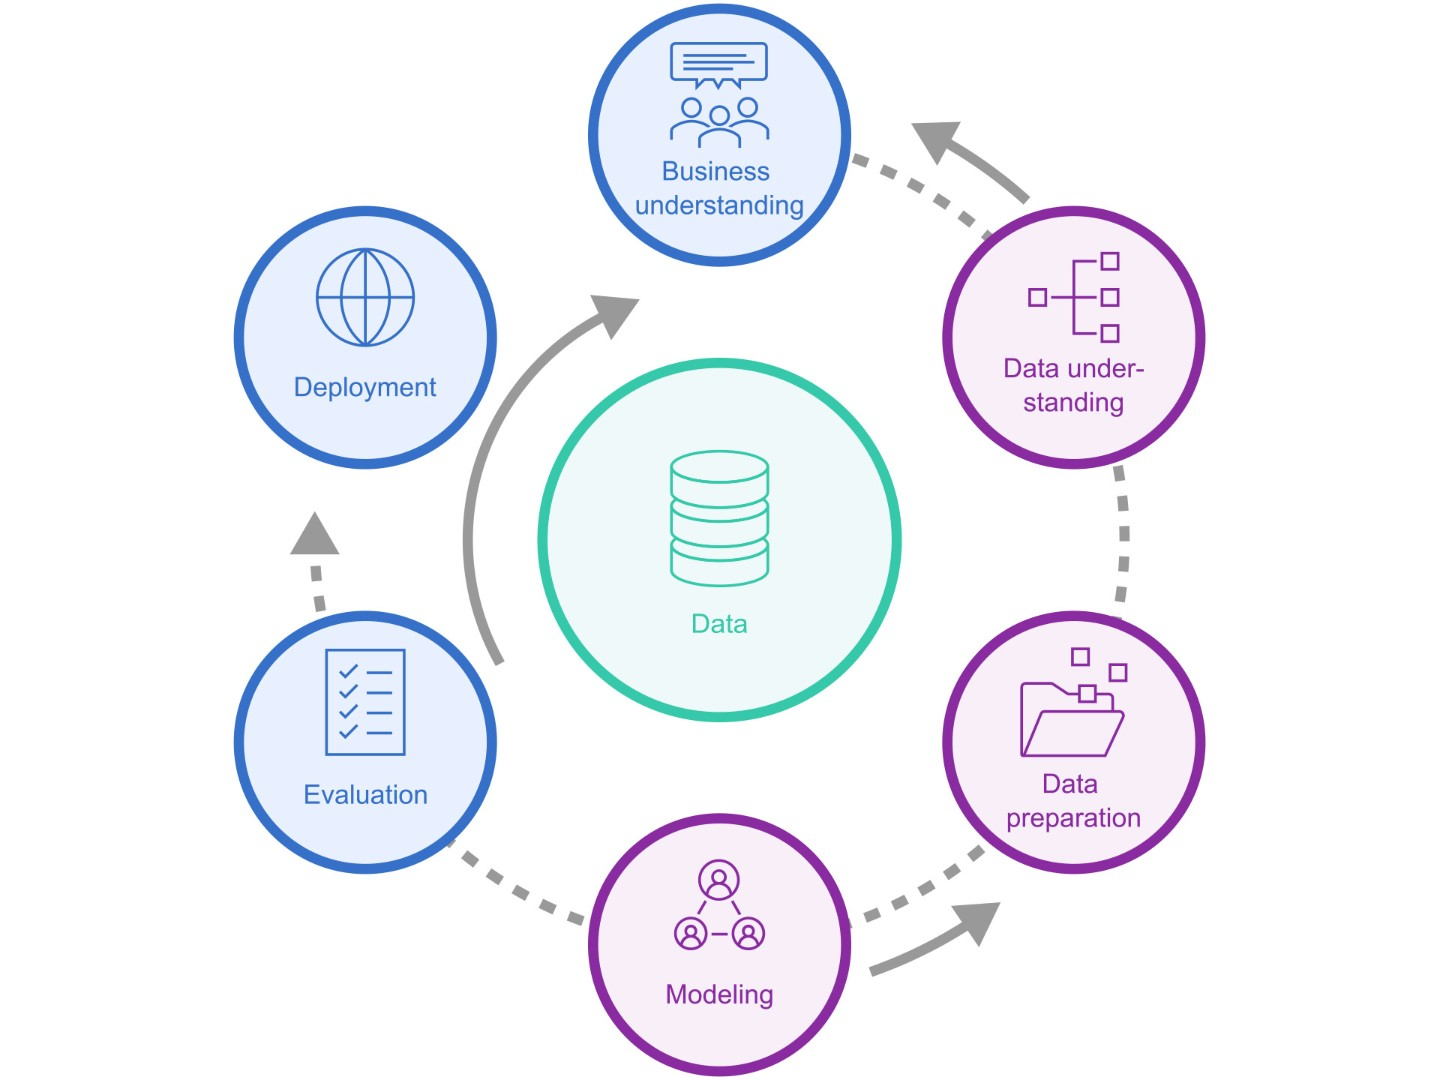
\includegraphics[width=0.7\textwidth]{image/crisp-dm-diagram.png}
  \caption{Siklus metodologi CRISP-DM \autocite{chapman2000}}
  \label{fig:crisp-dm}
\end{figure}

Metodologi CRISP-DM yang diadaptasi untuk pengembangan sistem rangkuman otomatis ini terdiri dari enam fase berikut:

\begin{enumerate}
\item \textbf{\textit{Business Understanding}}: Memahami kebutuhan komunitas finansial Telegram dan mendefinisikan tujuan proyek dari perspektif bisnis, yaitu mereduksi \textit{information overload} melalui rangkuman otomatis.

\item \textbf{\textit{Data Understanding}}: Mengumpulkan dan menganalisis data pesan dari tiga grup Telegram target untuk memahami karakteristik, volume, dan pola komunikasi dalam komunitas.

\item \textbf{\textit{Data Preparation}}: Membersihkan, mentransformasi, dan mempersiapkan data pesan untuk pemrosesan NLP, termasuk normalisasi teks dan ekstraksi fitur linguistik.

\item \textbf{\textit{Modeling}}: Mengintegrasikan model NLP untuk analisis sentimen, ekstraksi entitas, identifikasi topik, dan generasi rangkuman menggunakan \textit{large language model}.

\item \textbf{\textit{Evaluation}}: Mengevaluasi kualitas rangkuman yang dihasilkan sistem melalui metrik objektif dan \textit{feedback} subjektif dari pengguna komunitas.

\item \textbf{\textit{Deployment}}: Mengimplementasikan sistem secara operasional dalam komunitas, termasuk penjadwalan otomatis dan penyampaian rangkuman periodik ke kanal Telegram.
\end{enumerate}

Penjelasan detail mengenai aktivitas dan keluaran dari setiap fase metodologi CRISP-DM dalam konteks penelitian ini akan diuraikan lebih lanjut pada Bab III (Analisis dan Perancangan Sistem).
